\documentclass[main]{subfiles}
\begin{document}
\chapter{简介}\label{chp:intro}

子空间聚类问题来自于很多实际的应用,包括运动轨迹分离~\cite{costeira1998motion_seg},
人脸识别~\cite{basri2003lambertianface},网络跳点计数~\cite{eriksson2011high_rankMC},
电影评分~\cite{zhang2012RecSys} 以及社交图谱~\cite{xu2011graphclustering}。
这些应用产生的高维数据通常可以看作是从多个混合的低维线性子空间的采样(如图\ref{fig:Union_of_sub_model}所示)。
子空间聚类就是在不知道类别信息的情况下,将这些数据按照它们原本所属的子空间重新聚合,
并且恢复出数据中隐含的子空间结构。
对应于上面所述的应用,子空间聚类能根据运动轨迹分离刚体,判断哪些面部照片来自同一个人,哪些网络
节点属于一个子网,给出观影兴趣相似的用户以及发现社交网络中隐含的人际关系。

\begin{figure}
  \centering
  % Requires \usepackage{graphicx}
  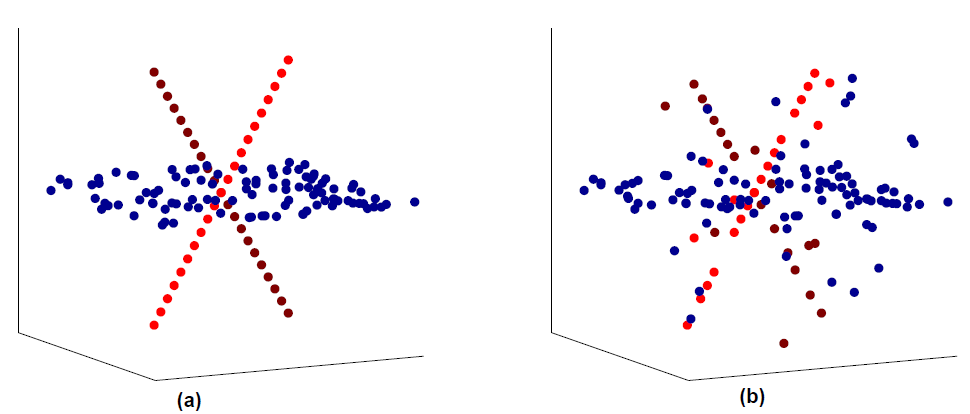
\includegraphics[width=0.8\linewidth]{pics/Union_of_Subspace.png}\\
  \caption{采样于三个子空间的无噪音 (a) 和有噪音 (b) 数据}\label{fig:Union_of_sub_model}
\end{figure}

过去十年,很多人关注子空间聚类问题,并且提出了许多算法,包括 Expectation-Maximization 类型的局部优化算法,
比如 K-plane~\cite{bradley2000k-plane} 和 Q-flat~\cite{tseng2000qflat},代数方法,比如
广义主成分分析(Generalized Principal Component Analysis)~\cite{vidal2005gpca},
矩阵分解方法~\cite{costeira1998motion_seg,costeira2000multibody_factorization},基于谱聚类的方法
~\cite{lauer2009spectral,chen2009spectral},自底向上的局部采样方法~\cite{yan2006LSA,rao2008motion},
以及基于凸优化的方法,比如低秩表示(Low Rank Representation)~\cite{liu2010lrr_icml,liu2013LRR}
和稀疏子空间聚类(Sparse Subspace Clustering)~\cite{elhamifar2009ssc,elhamifar2012ssc_journal}。
这些算法中,SSC是最优秀的之一,尤其当数据有噪音时,表现地相对稳健和鲁棒,例如在运动分割领域的
Hopkins155~\cite{tron2007benchmark,elhamifar2009ssc}测试集上,SSC是目前公认的表现最好的算法,
并且当类别增多时,它表现得比 LRR 更好~\cite{elhamifar2012ssc_journal}。

SSC算法的关键是将每个数据点用其他点线性表示,由于每个点都在一个低维子空间中,则一定存在一个相对稀疏的表示,
只用到同一个子空间中的点。如果把系数大小看作两个点的连接权重,我们可以得到一个无向图,再对这个图进行谱聚类,
即可将不同子空间的点分开。如果用第~\ref{chp:prob_setup}节中的符号描述,那么无噪音和有噪音的 SSC 分别求解
\begin{align*}
  \min_{c_i} \|c_i\|_1\quad s.t.\quad X_i=X_{\{i\}^c}c_i, \\
  \min_{c_i} \|c_i\|_1+\frac{\lambda}{2}\|X_i-X_{\{i\}^c}c_i\|^2,
\end{align*}
$X_i$ 表示数据矩阵的第$i$ 列, $c_i$ 是$X_i$ 用其他所有点表示的系数,我们希望其非零元素对应的数据点都和 $x_i$ 在同一个子空间。
对于仿射子空间,SSC 同样适用,只需要加上 $c_i = i$的限制。

\begin{algorithm}[tb]
  \caption{Sparse Subspace Clustering}
  \label{alg:SSC}
  \begin{algorithmic}
    \State {\bfseries Input:}
    Data points as columns in $X\in \mathbb{R}^{n\times N}$.
    \State{1. } For each data point $x_i$, solve
    \begin{align}\label{eq:SSC}
      \min_{c_i} \; \|c_i\|_1 \quad s.t. \quad &x_i=X_{-i}c_i
    \end{align}
    \State{2. } Let $C:=[c_1,...,c_N]$. Form affinity graph $G$ that is represented by adjacency matrix $W=|C|+|C|^T$.
    \State{3. } Estimate the number of subspace by finding the largest eigenvalue gap of normalized Laplacian of $G$ via
    $$\hat{L}=N-\underset{i=1,...,N-1}{\text{argmax}}\; \sigma_i-\sigma_{i+1}$$
    \State{4. } 对 $G$ using $\hat{L}$.
    \State {\bfseries Output:} Subspace partitions $\mathcal{X}_1,...,\mathcal{X}_{\hat{L}}$
  \end{algorithmic}
\end{algorithm}

然而,在 SSC 中,我们每次只考虑一个点相对于其他点的表示,
比较容易受到噪音和异常点的干扰。如果我们预先知道点$A,B,C$
属于同一类,然后寻找其他几个点能同时表示$A,B,C$,这无疑比
单独考虑$A$ 或 $B$ 或 $C$ 更稳健。另一方面,在SSC 模型中,
我们只是要求稀疏尽量稀疏,如此产生的邻接矩阵,不一定能在
接下来的谱聚类中有比较好的可分性。如果我们能让表示向量的非零元
集中在某些位置,那么邻接矩阵将具有更好的结构(具体可见第\ref{chp:experiments}节)

基于上面的考虑,本文提出了一种新的子空间聚类方法,它的核心内容有两步:
首先根据点的空间信息,将某些很可能是一类的点聚在一起。然后我们在剩余的
点中,寻找能同时表示它们的点,进而构造邻接矩阵。
coefficients of these exemplar data points are likely to be
seen significant across different representations for many
data points. But on the other hand, the representation for
each data point still needs to respect the sparse subspace
assumption. 事实上,压缩感知中的 joint sparse 模型[1]  [17] 很好地满足了我们的需求。
另一方面

Effort has been made to explain the practical success of SSC by analyzing the noiseless version. \cite{elhamifar2010ssc_icassp} show that under certain conditions, \emph{disjoint} subspaces (i.e., they are not overlapping) can be exactly recovered.
%Similar guarantee, under stronger ``independent subspace'' condition, was provided for LRR in a much earlier analysis\cite{kanatani2001motion}.
A recent geometric analysis of SSC~\cite{soltanolkotabi2011geometric} broadens the scope of the results significantly to the case when subspaces can be overlapping. However, while these analyses advanced our understanding of SSC, one common drawback
is that data points are assumed to be lying {\em exactly} on the subspaces. This assumption can hardly be satisfied in practice. For example, motion trajectories data are only {\em approximately} of rank-4 due to perspective distortion of camera, tracking errors and pixel quantization~\cite{costeira1998motion_seg}; similary, face images are   not precisely of rank-9 since human faces are at best {\em approximated} by a convex body~\cite{basri2003lambertianface}.

In this paper, we address this problem and provide a theoretical analysis of SSC with noisy or corrupted data. Our main result shows that a modified version of SSC (see Eq. \eqref{eq:Lasso}) succeeds when the magnitude of noise does not exceed a threshold determined by a geometric gap between the \emph{inradius} and the \emph{subspace incoherence} (see below for precise definitions). This complements the result of \cite{soltanolkotabi2011geometric} that shows the same geometric gap determines whether SSC succeeds for the noiseless case. Indeed,  when the noise vanishes, our results reduce to the noiseless case results of \cite{soltanolkotabi2011geometric}.

While our analysis is based upon the geometric analysis of \cite{soltanolkotabi2011geometric}, the analysis is more involved: In SSC, sample points are used as the dictionary for sparse recovery, and therefore noisy SSC requires analyzing a noisy dictionary.
%This is a hard problem and we are not aware of any previous study that proposed guarantee in the case of noisy dictionary except \cite{loh2012high} in the high-dimensional regression problem.
We also remark that our results on noisy SSC are {\em exact}, i.e., as long as the noise magnitude is smaller than a threshold, the recovered subspace clusters are {\em correct}.
This is in sharp contrast to the majority of previous work on structure recovery for noisy data where stability/perturbation bounds are given~--~i.e., the obtained solution is {\em approximately} correct, and the approximation gap goes to zero only when the noise diminishes.

Lastly, we remark that an independently developed work \cite{soltanolkotabi2013robust} analyzed the same algorithm {\em under a statistical model} that generates the data. In contrast, our main results focus on the cases when the data are deterministic. Moreover, when we specialize our general result to the same statistical model, we show that we can handle a significantly larger amount of noise under certain regimes.

%{\color{red}[Is this sentence too strong, since ours is stronger in some situations, and weaker in others]}. We will describe the differences in the next section.


%Then in Section~\ref{sec:ADMM_matrix-LASSO-SSC} we derive a fast numerical solver for the matrix version of our algorithm.
\section{Related works}\label{sec:RelatedWorks}
In this section, we review  previous and ongoing theoretical studies on the problem of subspace clustering.

\subsection{Nominal performance guarantee for noiseless data}
Most previous analyses concern about the nominal performance of a particular subspace clustering algorithm with noiseless data. The focus is to relax the assumptions on the underlying subspaces and data generation.

A number of methods have been shown working under the \emph{independent subspace} assumption including the early factorization-based methods \cite{costeira1998motion_seg,kanatani2001motion}, LRR~\cite{liu2010lrr_icml} and the initial guarantee of SSC~\cite{elhamifar2009ssc}. Recall that the data points are drawn from a union of subspaces, the \emph{independent subspace } assumption requires each subspace to be linearly independent to the {\em span} of all other subspaces. Equivalently, this assumption requires the sum of each subspace's dimension to be equal to the dimension of the span of all subspaces. For example, in a two dimensional plane, one can only have 2 independent lines. If there are three lines intersecting at the origin, even if each pair of the lines are independent, they are not considered independent as a whole.

\emph{Disjoint subspace} assumption only requires pairwise linear independence, and hence is more meaningful in practice. To the best of our knowledge, only GPCA~\cite{vidal2005gpca} and SSC~\cite{elhamifar2010ssc_icassp,elhamifar2012ssc_journal} have been shown to provably handle the data under \emph{disjoint subspace} assumption. GPCA however is not a polynomial time algorithm. Its computational complexity increases exponentially with respect to the number and dimension of the subspaces.

\cite{soltanolkotabi2011geometric} developed a geometric analysis that further extends the performance guarantee of SSC, and in particular it covers some cases when the underlying subspaces are slightly \emph{overlapping}, meaning that two subspaces can even share a basis. The analysis reveals that the success of SSC relies on the difference of two geometric quantities (inradius $r$ and incoherence $\mu$) to be greater than $0$, which leads to by far the most general and strongest theoretical guarantee for noiseless SSC. A summary of these assumptions on the subspaces and their formal definition are given in Table~\ref{tab:subspaces}.
\begin{table}
  \centering
\begin{tabular}{|l|c|}
  \hline
  % after \\: \hline or \cline{col1-col2} \cline{col3-col4} ...
  Independent Subspaces & $\dim\left[\cS_1\otimes...\otimes \cS_L\right] = \sum_{\ell=1}^L \dim\left[\cS_\ell\right]  $.  \\\hline
  Disjoint Subspaces &  $\cS_\ell\cap \cS_k =\mathbf{0}$ for all $\{(\ell,k)|\ell\neq k\}$.\\\hline
  Overlapping Subspaces & No points lies in $\cS_\ell\cap \cS_k$ for any $\{(\ell,k)|\ell\neq k\}$.\\
  \hline
\end{tabular}
\caption{Comparison of conditions on the underlying subspaces.}\label{tab:subspaces}
\end{table}



\subsection{Robust performance guarantee}

Previous studies of the subspace clustering under noise have been mostly empirical. For instance, factorization, spectral clustering and local affinity based approaches, which we mentioned above, are able to produce a (sometimes good) solution even for noisy real data. Convex optimization based approaches like LRR and SSC can be naturally reformulated as a robust method by relaxing the hard equality constraints to a penalty term in the objective function. In fact, the superior results of SSC and LRR on motion segmentation and face clustering data are produced using the robust extension in \cite{elhamifar2009ssc} and \cite{liu2010lrr_icml} instead of the well-studied noiseless version.

As of writing, there have been very few subspace clustering methods that is guaranteed to work when data are noisy.  Besides the conference version of the current paper~\cite{wang2013noisy}, an independent work \cite{soltanolkotabi2013robust} also analyzed SSC under noise. Subsequently, there has been noisy guarantees for other algorithms, e.g., thresholding based approach \cite{heckel2013noisy} and
orthogonal matching pursuit \cite{dyer2013greedy}.
 %proposed and analyzed a thresholding based algorithm for subspace clustering, where recovery under noise is proven effective.

The main difference between our work and \cite{soltanolkotabi2013robust} is that our guarantee works for a more general set of problems when the data and noise may not be random, whereas the key arguments in the proof in \cite{soltanolkotabi2013robust} relies on the assumption that data points are uniformly distributed on the unit sphere within each subspace, which corresponds to the ``semi-random model'' in our paper.
As illustrated in \cite[Figure~9~and~10]{elhamifar2012ssc_journal}, the semi-random model is not a good fit for both the motion segmentation and the face clustering datasets, as in these datasets there is a fast decay in the singular values of each subspace.  The uniform distribution assumption becomes even harder to justify as the dimension $d$ of each subspace gets larger --- a regime where the analysis in \cite{soltanolkotabi2013robust} focuses on.

Moreover, with a minor modification in our analysis that sharpens the bound of the tuning parameter that ensures the solution is non-trivial, we are able to get a result that is stronger than \cite{soltanolkotabi2013robust} in cases when the dimension of each subspace $d\leq O(\sqrt{n})$ \footnote{Admittedly, \cite{soltanolkotabi2013robust} obtained better noise-tolerance than the comparable result in our conference version \cite{wang2013noisy}. }. This result extends the provably guarantee of SSC to a setting where the signal to noise ratio (SnR) is allowed to go to $0$ as the ambient dimension gets large. In summary, we compare our results in terms of the level of noise that can be provably tolerated in Table~\ref{tab:comparison}. These comparisons are in the same setting modulo some slight differences in the noise model and successful criteria. It is worth noting that when $d>O(\sqrt{n})$, \cite{soltanolkotabi2013robust}'s bound is sharper. We will provide more details in the Appendix.


%{\color{red} [Do we want to say more on the rate comparison, i.e., when $n>d^2$ our result is stronger and vice versa?]}

%Requiring the solution to be non-trivial v.s. requiring the solution to have $\Omega(d/\log(N))$ entries.


\begin{table}
\centering
\small{
\begin{tabular}{|p{2.2in}|p{1.05in}|p{1in}|p{1in}|p{1.2in}|}
  \hline
  % after \\: \hline or \cline{col1-col2} \cline{col3-col4} ...
   & This paper & \cite{wang2013noisy} & \cite{soltanolkotabi2013robust} \\\hline %\hhline{|=|=|=|=|}
  Fully deterministic & $O(r(r-\mu))$ & $O(r(r-\mu))$ & N.A.  \\\hline
  Deterministic + random noise & $O((n/d)^{\frac{1}{4}}(r-\mu))$ & $O(r-\mu)$ & N.A.   \\\hline
  Semi-random data + random noise & $O\left(\frac{n^{\frac{1}{4}}}{\sqrt{d}}(1-\frac{\text{aff}}{\sqrt{d}})\right)$ & $O\left(\frac{1}{\sqrt{d}}(1-\frac{\text{aff}}{\sqrt{d}})\right)$ & $O\left(1-\frac{\text{aff}}{\sqrt{d}}\right)$  \\\hline
    Fully-random data + random noise & $O\left(\frac{n^{\frac{1}{4}}}{\sqrt{d}}(1-\frac{\sqrt{d}}{\sqrt{n}})\right)$ & $O\left(\frac{1}{\sqrt{d}}(1-\frac{\sqrt{d}}{\sqrt{n}})\right)$ & $O\left(1-\frac{\sqrt{d}}{\sqrt{n}}\right)$  \\
  \hline
\end{tabular}
}
\caption{Comparison of the level of noise tolerable for noisy subspace clustering methods. Note that ``$\mathrm{aff}$'' is the ``unnormalized'' affinity defined in \cite{soltanolkotabi2011geometric}}.\label{tab:comparison}
\end{table}

%\begin{table}\label{tab:comparison}
%\centering
%\small{
%\begin{tabular}{|p{1in}|p{1.05in}|p{1in}|p{1in}|p{1.2in}|}
%  \hline
%  % after \\: \hline or \cline{col1-col2} \cline{col3-col4} ...
%   & This paper & \cite{wang2013noisy} & \cite{soltanolkotabi2013robust} & \cite{heckel2013noisy,heckel2013robust}\\\hline %\hhline{|=|=|=|=|=|}
%  Fully deterministic & $O(r(r-\mu))$ & $O(r(r-\mu))$ & N.A. & N.A.  \\\hline
%  Deterministic + random noise & $O((n/d)^{\frac{1}{4}}(r-\mu))$ & $O(r-\mu)$ & N.A. & N.A.  \\\hline
%  Semi-random model + random noise & $O\left(\frac{n^{\frac{1}{4}}}{\sqrt{d}}(1-\frac{\text{aff}}{\sqrt{d}})\right)$ & $O\left(\frac{1}{\sqrt{d}}(1-\frac{\text{aff}}{\sqrt{d}})\right)$ & $O\left(1-\frac{\text{aff}}{\sqrt{d}}\right)$ & $O\left(\left(n/d\right)^{\frac{1}{4}}(1-\frac{\text{aff}}{\sqrt{d}})\right)$ \\\hline
%    Fully random model + random noise & $O\left(\frac{n^{\frac{1}{4}}}{\sqrt{d}}(1-\frac{\sqrt{d}}{\sqrt{n}})\right)$ & $O\left(\frac{1}{\sqrt{d}}(1-\frac{\sqrt{d}}{\sqrt{n}})\right)$ & $O\left(1-\frac{\sqrt{d}}{\sqrt{n}}\right)$ & $O\left(\left(n/d\right)^{\frac{1}{4}}(1-\frac{\sqrt{d}}{\sqrt{n}})\right)$ \\
%  \hline
%\end{tabular}
%}
%\caption{Comparison of the level of noise tolerable for noisy subspace clustering methods}
%\end{table}



%
%These results differs from ours in several ways:
%\begin{enumerate}
%  \item \textbf{Model of analysis}: Our main contributions include a guarantee that requires no probabilistic assumptions on the data generation and works for potentially adversarial noise, while the result in \cite{soltanolkotabi2013robust} relies on random sampling of data in each subspace and can handle only stochastic noise. Indeed, a guarantee for deterministic data is listed as future works in \cite{soltanolkotabi2013robust}.
%  \item \textbf{Results}: Our results in the semi-random model is directly comparable to the main theoretical results in \cite[Theorem~3.1~and~3.2]{soltanolkotabi2013robust}. It appears that their results focus on a high subspace dimension paradigm (large $d$) and becomes less meaningful in the more common cases when the underlying dimension of each subspace is low (see Table~\ref{tab:low_rank}). In particular, the lower bound in their Theorem~3.2 is can become meaninglessly small when $d$ is small. Moreover, the failure probability may not diminish in the cases when $d$ is small due to the $6 e^{-\gamma d}$ term. Right on the contrary, our results are stronger when $d$ is smaller, which are consistent with the simulation in Section~\ref{sec:experiments}.
%  \item \textbf{Proof techniques}:
%      The difference in the results is perhaps due to the fact that \cite{soltanolkotabi2013robust} requires each subspace's data to obey the Restricted Isometry Property (RIP)\footnote{The requirement of RIP is hidden in the proof of Lemma~8.3 in \cite{soltanolkotabi2013robust}, which is critical for their main results \cite[Theorem~3.1~and~3.2]{soltanolkotabi2013robust}.}~\cite{candes2008RIP}, while ours does not need it. When the number of data increases, it is more likely that multiple similar data points occur, which makes RIP prone to fail. On the other hand, in the subspace clustering problem (in particular SSC), more data samples we have in each subspace should intuitively be good since the representation of the underlying subspace is better (a larger inradius $r$). That is why we suspect RIP may not capture the intrinsic properties of the problem.
%%
%%  \item \textbf{Proof techniques}: The results of \cite{soltanolkotabi2013robust} requires each subspace's data to obey Restricted Isometry Property (RIP)\footnote{The requirement of RIP is hidden in the proof of Lemma~8.3 in \cite{soltanolkotabi2013robust}, which is critical for their main results \cite[Theorem~3.1~and~3.2]{soltanolkotabi2013robust}.}~\cite{candes2008RIP}, while ours does not need it. When the number of data increases, it is more likely that multiple similar data points occur, which makes RIP prone to fail. On the other hand, in the subspace clustering problem (in particular SSC), more data samples we have in each subspace should intuitively be good since the representation of the underlying subspace is better (a larger inradius $r$). That is why we suspect RIP may not capture the intrinsic properties of the problem.
%%  \item \textbf{Failure probability}: The failure probability of \cite{soltanolkotabi2013robust} contains to $6 e^{-\gamma d}$ and $13/N$ for some small constant $\gamma$. Note that $d$ is the dimension of each subspace and $N$ is the total number of data points. The failure probability may not diminish in the cases when $d$ is small (say if $\gamma=1/4$ and $d=4$). Also note that the result is stated for a single column. Because of the $13/N$ term, there is no simple way to guarantee that the probability of all $N$ columns is small using union bound. Quite on the contrary, our results for the same model (Theorem~\ref{thm:semirandom}) has diminishing failure probability for all $N$ data points, and is stronger for smaller $d$.
%%  \item \textbf{Algorithm}: A more apparent difference is on the algorithm. The key novelty of \cite{soltanolkotabi2011geometric} is to propose the two-pass mechanism and adaptively choosing a good trade-off parameter for each data point. While it may be advantages to choose a different parameter for each data point, our algorithm uses a uniform parameter for all data points. Instead of a procedure to tune the parameter, we provide a range of valid parameter in analytic form.
%\end{enumerate}





Lastly, we note that the notion of robustness in this paper is confined to the noise/arbitrary corruptions added to the legitimate data. It is not the robustness against outliers in the data, unless otherwise specified. Handling outliers is a completely different problem. Solutions have been proposed for LRR in \cite{liu2012aistats} by decomposing a $\ell_{2,1}$ norm column-wise sparse components and for SSC in \cite{soltanolkotabi2011geometric} by objective value thresholding. However these results require non-outlier data points to be free of noise, therefore are not comparable to the study in this paper.

\end{document}
